\documentclass[border=4pt]{standalone}
\usepackage{tikz}
\usetikzlibrary{arrows.meta,positioning,calc,fit,backgrounds,patterns,shapes.geometric}
\usepackage{amsmath,amssymb}
\usepackage{mathptmx}
\definecolor{lost}{HTML}{C2362D}
\definecolor{kept}{HTML}{17875A}
\definecolor{evid}{HTML}{3056D3}
\definecolor{ink}{HTML}{1D1D1F}
\definecolor{muted}{HTML}{6E6E73}
\tikzset{
  box/.style={draw=ink!70, rounded corners=2pt, align=center, fill=white, inner sep=4pt, font=\footnotesize},
  arr/.style={-{Stealth[length=2mm]}, draw=ink!70, line width=0.6pt},
  grp/.style={draw=muted!60, dashed, rounded corners=4pt, inner sep=7pt},
  lossbox/.style={draw=lost!80, fill=lost!6, text=lost!85!black, rounded corners=2pt, align=left, font=\footnotesize, inner sep=4pt},
  fixbox/.style={draw=kept!80, fill=kept!7, text=kept!65!black, rounded corners=2pt, align=left, font=\footnotesize, inner sep=4pt},
  dec/.style={diamond, aspect=2.2, draw=ink!70, fill=evid!6, align=center, font=\footnotesize, inner sep=1.5pt},
  lbl/.style={font=\footnotesize\bfseries, text=ink},
}

\begin{document}
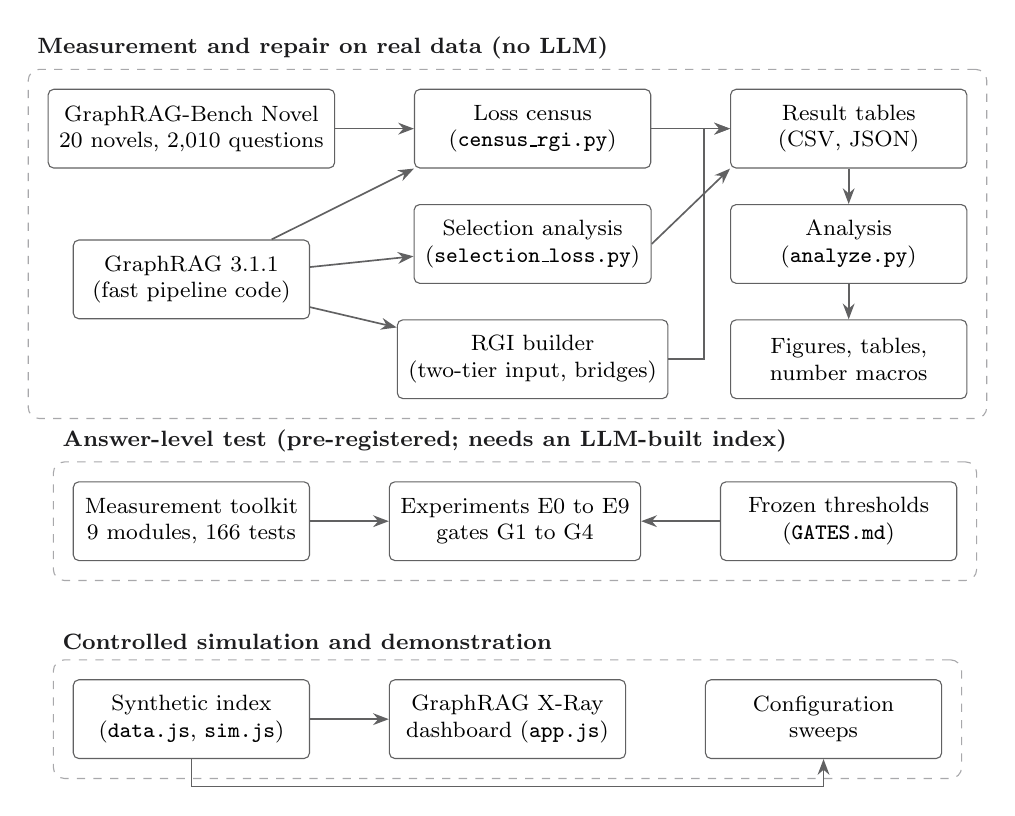
\begin{tikzpicture}[node distance=0.45cm]
\node[box, minimum width=3.0cm, minimum height=1.0cm] (data) {GraphRAG-Bench Novel\\20 novels, 2,010 questions};
\node[box, minimum width=3.0cm, minimum height=1.0cm, below=0.9cm of data] (gr) {GraphRAG 3.1.1\\(fast pipeline code)};
\node[box, minimum width=3.0cm, minimum height=1.0cm, right=1.0cm of data] (census) {Loss census\\(\texttt{census\_rgi.py})};
\node[box, minimum width=3.0cm, minimum height=1.0cm, below=0.45cm of census] (sel) {Selection analysis\\(\texttt{selection\_loss.py})};
\node[box, minimum width=3.0cm, minimum height=1.0cm, below=0.45cm of sel] (rgi) {RGI builder\\(two-tier input, bridges)};
\node[box, minimum width=3.0cm, minimum height=1.0cm, right=1.0cm of census] (res) {Result tables\\(CSV, JSON)};
\node[box, minimum width=3.0cm, minimum height=1.0cm, below=0.45cm of res] (an) {Analysis\\(\texttt{analyze.py})};
\node[box, minimum width=3.0cm, minimum height=1.0cm, below=0.45cm of an] (out) {Figures, tables,\\number macros};
\draw[arr] (data) -- (census); \draw[arr] (gr) -- (census.south west); \draw[arr] (gr) -- (sel); \draw[arr] (gr) -- (rgi);
\draw[arr] (census) -- (res); \draw[arr] (sel.east) -- (res.south west); \draw[arr] (rgi.east) -- ++(0.45,0) |- (res.west);
\draw[arr] (res) -- (an); \draw[arr] (an) -- (out);
\begin{scope}[on background layer]
\node[grp, fit=(data)(gr)(census)(sel)(rgi)(res)(an)(out), label={[lbl, anchor=south west]north west:Measurement and repair on real data (no LLM)}] (g1) {};
\end{scope}
\node[box, minimum width=3.0cm, minimum height=1.0cm] (kit) at ($(gr |- rgi.south)+(0,-1.55)$) {Measurement toolkit\\9 modules, 166 tests};
\node[box, minimum width=3.0cm, minimum height=1.0cm, right=1.0cm of kit] (gates) {Experiments E0 to E9\\gates G1 to G4};
\node[box, minimum width=3.0cm, minimum height=1.0cm, right=1.0cm of gates] (pre) {Frozen thresholds\\(\texttt{GATES.md})};
\draw[arr] (kit) -- (gates); \draw[arr] (pre) -- (gates);
\begin{scope}[on background layer]
\node[grp, fit=(kit)(gates)(pre), label={[lbl, anchor=south west]north west:Answer-level test (pre-registered; needs an LLM-built index)}] (g2) {};
\end{scope}
\node[box, minimum width=3.0cm, minimum height=1.0cm, below=1.5cm of kit] (simd) {Synthetic index\\(\texttt{data.js}, \texttt{sim.js})};
\node[box, minimum width=3.0cm, minimum height=1.0cm, right=1.0cm of simd] (ui) {GraphRAG X-Ray\\dashboard (\texttt{app.js})};
\node[box, minimum width=3.0cm, minimum height=1.0cm, right=1.0cm of ui] (sw) {Configuration\\sweeps};
\draw[arr] (simd) -- (ui); \draw[arr] (simd.south) -- ++(0,-0.35) -| (sw.south);
\begin{scope}[on background layer]
\node[grp, fit=(simd)(ui)(sw), label={[lbl, anchor=south west]north west:Controlled simulation and demonstration}] (g3) {};
\end{scope}
\end{tikzpicture}
\end{document}
